%
% Created       : 2014 Jul 21 (Mon) 10:47:41 by Harold Carr.
% Last Modified : 2014 Jul 22 (Tue) 19:00:39 by Harold Carr.
%

% \documentclass[convert={density=300,size=1080x800,outext=.png}]{standalone}
% \documentclass[convert={density=300,outext=.png}]{standalone}
\documentclass[convert={density=175,outext=.png}]{standalone}

\usepackage{tikz}
\usetikzlibrary{matrix,arrows}

\begin{document}

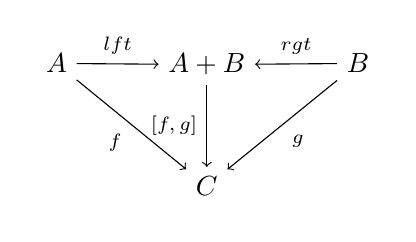
\begin{tikzpicture}[descr/.style={fill=white,inner sep=2.5pt}]
\matrix (m) [matrix of math nodes, row sep=3em, column sep=3em]
{ A & A + B & B \\
    &   C   &   \\
};
\path[->,font=\scriptsize]
(m-1-1) edge node[auto]      {$ lft    $}  (m-1-2)
(m-1-3) edge node[auto,swap] {$ rgt    $}  (m-1-2)
(m-1-1) edge node[auto,swap] {$ f      $}  (m-2-2)
(m-1-2) edge node[auto,swap] {$ [f, g] $}  (m-2-2)
(m-1-3) edge node[auto]      {$ g      $}  (m-2-2)
;
\end{tikzpicture}

\end{document}

% End of file.
